\setcounter{ExampleCounter}{1}
Later in this chapter, we'll want to find where two lines intersect.
\begin{center}
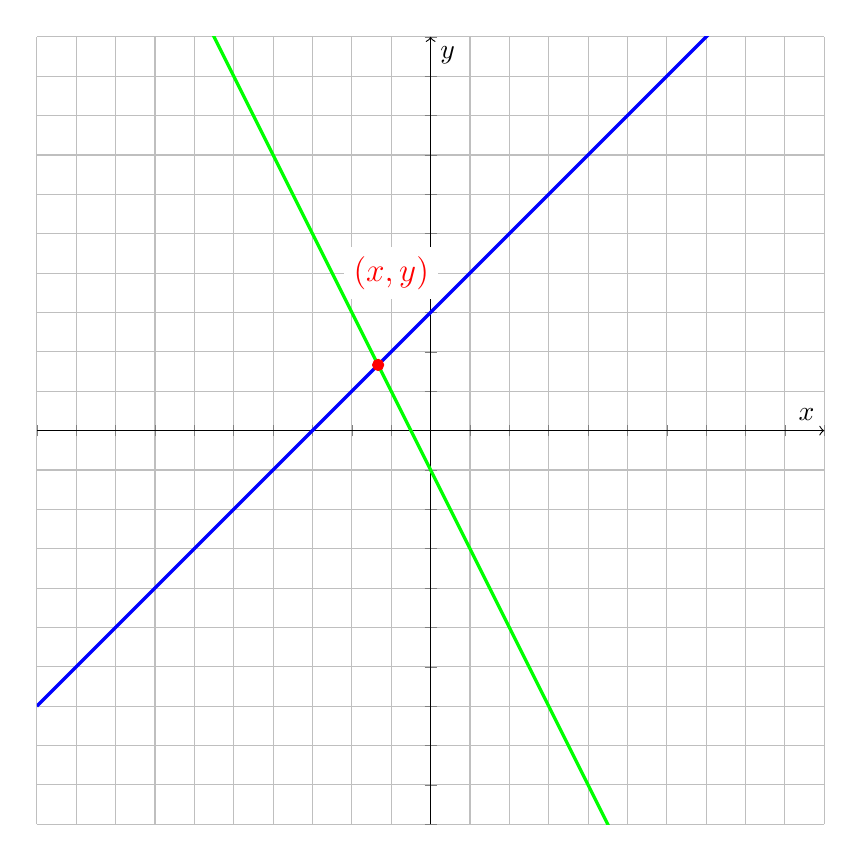
\begin{tikzpicture}
\begin{axis}[
    xmin=-10, xmax=10,
    ymin=-10, ymax=10,
    axis lines=center,
    axis on top=false,
    domain=0:1,
    x=0.5cm,
    y=0.5cm,
    xtick={-10,-9,...,10},
    xticklabels={},
    ytick={-10,-9,...,10},
    yticklabels={},
    axis lines=middle,
    axis line style={->},
    xlabel={$x$},
    ylabel={$y$},
    grid=major
    ]
    \addplot [only marks,color=red] table {
	-1.333 1.667
	};
	\draw [yshift=12.5cm,xshift=4.5cm] node [fill=white] {\large\color{red}$(x,y)$};
	\addplot [very thick,blue,domain=-10:10] {x+3};
	\addplot [very thick,green,domain=-10:10] {-2*x-1};
\end{axis}
\end{tikzpicture}
\end{center}

When we solve this, what we are finding is the point $(x,y)$ that lies on both lines.

\begin{formula}{Solving a System of Linear Equations}
Solving a system of linear equations means finding an $x,y$ pair that fits both equations at once.
\end{formula}

To see this, take the system of equations (pair of lines) shown below.
\begin{align*}
2x+y &= 5\\
x-3y &= -8
\end{align*}
We can show that the point $(1,3)$ is the point where they cross by substituting it into both equations and seeing that it fits into both of them:
\begin{center}
\begin{tabular}{r l}
$2(1)+(3)=5$ & TRUE\\
$(1)-3(3)=-8$ & TRUE
\end{tabular}
\end{center}
You can check other points by substituting them into these two equations, but you won't find any other combination of $x$ and $y$ that satisfies the system.  For instance, $(2,1)$ is a solution to the first equation, but not to the second.

That illustrates how we can check a proposed solution (intersection point of two lines), but it doesn't show how to \emph{find} the solution.  In this section, we'll see three methods for solving systems like this: one graphical and two algebraic.
\vfill
\pagebreak

\subsection{Solving by Graphing}
If we can graph the two lines and simply spot where they cross, we can check our answer by substituting it into the system.

\begin{example}[https://www.youtube.com/watch?v=ymuYIaGzWw8]{Solving a Linear System by Graphing}
Solve the following system of equations by graphing.
\begin{align*}
2x+y &= 5\\
x-3y &= -8
\end{align*}

\sol
Start by graphing the two lines, using one of the methods in the previous section.
\begin{center}
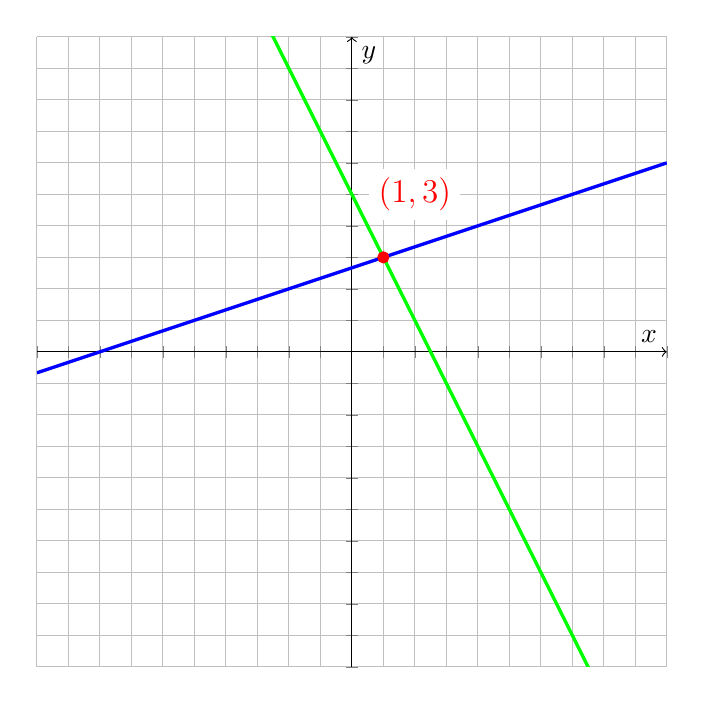
\begin{tikzpicture}
\begin{axis}[
    xmin=-10, xmax=10,
    ymin=-10, ymax=10,
    axis lines=center,
    axis on top=false,
    domain=0:1,
    x=0.4cm,
    y=0.4cm,
    xtick={-10,-9,...,10},
    xticklabels={},
    ytick={-10,-9,...,10},
    yticklabels={},
    axis lines=middle,
    axis line style={->},
    xlabel={$x$},
    ylabel={$y$},
    grid=major
    ]
    \addplot [only marks,color=red] table {
	1 3
	};
	\draw [yshift=8cm,xshift=4.8cm] node [fill=white] {\large\color{red}$(1,3)$};
	\addplot [very thick,blue,domain=-10:10] {x/3+8/3};
	\addplot [very thick,green,domain=-10:10] {-2*x+5};
\end{axis}
\end{tikzpicture}
\end{center}

It \emph{looks} like the lines cross at $(1,3)$, but maybe our lines aren't perfectly graphed, and maybe they cross at $(1.01,2.99)$.  To make sure that they cross at exactly $(1,3)$, we can substitute this point into both equations and make sure it is a solution to both.

\begin{center}
\begin{tabular}{r l}
$2(1)+(3)=5$ & TRUE\\
$(1)-3(3)=-8$ & TRUE
\end{tabular}
\end{center}
\end{example}

\begin{try}
Find the solution of the system of equations graphed below.
\begin{minipage}[b]{0.48\textwidth}
\begin{align*}
3x+2y &= 8\\
2x+2y &= 6
\end{align*}
\end{minipage}
\begin{minipage}{0.48\textwidth}
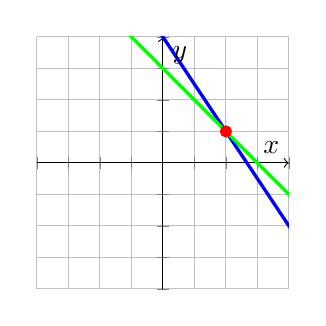
\begin{tikzpicture}
\begin{axis}[
    xmin=-4, xmax=4,
    ymin=-4, ymax=4,
    axis lines=center,
    axis on top=false,
    domain=0:1,
    x=0.4cm,
    y=0.4cm,
    xtick={-10,-9,...,10},
    xticklabels={},
    ytick={-10,-9,...,10},
    yticklabels={},
    axis lines=middle,
    axis line style={->},
    xlabel={$x$},
    ylabel={$y$},
    grid=major
    ]
    \addplot [only marks,color=red] table {
	2 1
	};
	\addplot [very thick,blue,domain=-10:10] {-3*x/2+4};
	\addplot [very thick,green,domain=-10:10] {-x+3};
\end{axis}
\end{tikzpicture}
\end{minipage}
\end{try}

As we noted, solving by graphing only works when we can easily spot the solution, and it happens to be nice round numbers.  In more general problems, we'll need to solve systems like this algebraically rather than graphically.

We have to algebraic ways to solve a system of linear equations, but both boil down to reducing the system of equations to a single equation with only one unknown--either $x$ or $y$.  Once we have that, we can solve the resulting equation and get half of the solution--one of the coordinates of the intersection--and use that half to get the other half.

\subsection{Solving by Substitution}
The first way that we'll reduce a system of two equations with two unknowns to a single equation with one unknown is by \textbf{substitution}.

Look at the system of equations below.
\begin{align*}
2x+3y &= 1\\
-2x+y &= 3
\end{align*}

Just focus on the first equation for a moment.  If we knew what $y$ was, we could substitute that into the first equation and get an equation that only involved $x$, which we could solve.  Unfortunately, we don't have a number for $y$ yet, but we \emph{do} know that $y$ is equal to $2x+3$.  How do we know this?  This piece of information comes from the previously ignored second equation:
\begin{align*}
&-2x+y=3 \\
&+2x \hspace{0.45in}+2x\\
\end{align*}
\[y=2x+3\]

Notice that if we substitute this \textit{expression} into the first equation, we'll have accomplished our goal of reducing the system to a single equation with one unknown (in this case, $x$).  Thus, simply replace $y$ in the first equation with $2x+3$:
\[2x+3(2x+3)=1\]
This is an equation we can solve, and if we do, we find that $x=-1.$

Here now is half the answer, the $x$-coordinate of the point where these two lines cross, but how do we find the $y$-coordinate?  Since this point lies on both lines, we can use either equation to find the $y$ that corresponds to this $x$, but we'll use the second equation, since we've done a little work to write it as $y=2x+3$, which makes it easy to find the $y$ that corresponds to $x=-1$:
\[y=2(-1)+3=1\]
The answer, then, is $x=-1$, $y=1$, which means that the two lines cross at the point $(-1,1)$.

Note that if we had plugged $x=-1$ into the first equation, we would have gotten the same result for $y$.  If we didn't, it would mean we had made a mistake in finding $x$.
\vspace{0.5in}

This example gives a blueprint for how to solve systems of linear equations by substitution.
\begin{proc}{Solving a Linear System by Substitution}
\begin{enumerate}
\item \marginnote{Pick the easier one}Solve one of the equations for one of the variables.
\item \marginnote{Substituting into the same equation won't do anything}Substitute that expression into the \emph{other} equation.
\item Solve the resulting equation for the variable that is left.
\item \marginnote{It's easier to substitute it into the one that you have solved for the other variable}Substitute that half of the answer into \emph{either} of the original equations to find the other half.
\end{enumerate}
\end{proc}
\vspace{0.4in}

Notice that this method gives you a lot of choice.  You can pick \emph{either} equation to solve for \emph{either} variable, and you can substitute the first half of the answer into \emph{either} equation to find the other half.  This lets you save some work if you look for one of the equations that is easier than the other to solve for one of the variables.
\pagebreak

\begin{example}[https://www.youtube.com/watch?v=ggZkBtnvLn0]{Solving by Substitution}
Solve the following system of equations by substitution.
\begin{align*}
2x+3y &= 11\\
x-4y &= 0
\end{align*}

\sol
It looks like the second equation is easier to solve for $x$, since $x$ only has a coefficient of 1 there.  Doing so gives \[x=4y.\]
We can now take this and plug $4y$ in for $x$ in the first equation:
\[2(4y)+3y=11 \longrightarrow 11y=11 \longrightarrow y=1\]
We've now got half of the answer, and we can substitute 1 for $y$ into either equation to find $x$, but we choose to use the rearranged form of the second equation:
\[x=4(1) = 4\]

The solution, or the point where the two lines cross, is therefore $\boxed{(4,1)}$.
\end{example}

\begin{try}
Use substitution to solve the following system of equations.
\begin{align*}
4x-y &= 5\\
3x+3y &= 15
\end{align*}
\end{try}

\begin{example}[https://www.youtube.com/watch?v=HqyePXNyhRU]{Solving by Substitution}
Use substitution to solve the following system of equations.
\begin{align*}
-4x+y &= -11\\
2x-3y &= 5
\end{align*}

\sol
We spot a lone $y$ in the first equation, so we solve the first equation for $y$ and get \[y=4x-11.\]
Substituting this into the second equation:
\[2x-3(4x-11)=5 \longrightarrow -10x=-28 \longrightarrow x=\frac{14}{5}\]

We can plug this half of the answer into the equation $y=4x-11$:
\[y=4\left(\frac{14}{5}\right)-11 = \frac{1}{5}\]

The point where the two lines cross is
\[\boxed{\left(\frac{14}{5},\frac{1}{5}\right)}\]
\end{example}

The answer in the last example is a clear instance where we could never have solved by graphing, at least by hand.
\pagebreak

\subsection{Solving by Elimination}
The other algebraic method we have to solve a linear system is called \textbf{elimination}.  The basic goal is still the same: to reduce the system to a single equation with one unknown.  What changes, though, is how we accomplish this.  We can use either substitution or elimination to solve any system of equations, but depending on the numbers used in a particular example, one may be easier than the other.

To illustrate solving by elimination, look at the following system of equations.
\begin{align*}
3x+2y &= 14\\
3x-2y &= 10
\end{align*}

The method of elimination uses the fact that we can add anything we want to one side of an equation as long as we add the same thing to the other side.

How does this help us?  Notice that the second equation says that $3x-2y$ and $10$ are the same, so we can add $3x-2y$ to the left side of the \emph{first} equation and 10 to its right side.  When we do so, the $2y$ and $-2y$ cancel each other:
\begin{alignat*}{1}
3x+2y &= 14\\
+3x-2y &= 10\\
\cline{0-1}
6x &= 24
\end{alignat*}
Thus, $x=4$, and substituting that into either one of the equations finds that $y=1$.

In that example, adding the equations made one of the variables cancel itself out, specifically because we had $2y$ in one equation and $-2y$ in the other.  What if the equations we're working with are not so compliant?

Take, for example, the system below.
\begin{align*}
2x-7y &= 2\\
3x+y &= -20
\end{align*}
Here, neither variable lines up so nicely, ready to be canceled, but if we multiply every term in the second equation by 7, the $y$'s will be ready to cancel.  Remember that we can multiply anything we want on one side of an equation as long as we multiply the same thing on the other side, so we're allowed to multiply the entire equation by 7, knowing that all we're changing is its form, not the actual equation.

If we do this, we get
\begin{align*}
2x-7y &= 2\\
21x+7y &= -140
\end{align*}

Now, when we add the two equations, $y$ is canceled, leaving \[23x=-138\] which we can solve to find that $x=-6$.  Finally, substituting that into either equation, we find that $y=-2$.

This leads to the following steps for solving a linear system by elimination.
\begin{proc}{Solving a Linear System by Elimination}
\begin{enumerate}
\item If necessary, arrange the equations so that the $x$'s and $y$'s line up vertically.
\item If necessary, multiply one or both of the equations by some constant that will make the coefficients of one of the variables opposites (same magnitude, but one positive and one negative).
\item Add the equations, canceling one of the variables.
\item Solve the resulting equation for the variable that is left.
\item Substitute that half of the answer into \emph{either} of the original equations to find the other half.
\end{enumerate}
\end{proc}

Notice that the last two steps are identical to the last two steps in the process of solving by substitution.
\pagebreak

\begin{example}[https://www.youtube.com/watch?v=fN5tA1onlu4]{Solving by Elimination}
Solve the following system of equations by elimination.
\begin{align*}
2x+3y &= -16\\
5x-10y &= 30
\end{align*}

\sol
Rather than multiplying one of the equations by a fraction in order to make the coefficients of $x$ or $y$ opposites, we'll multiply \emph{both} equations by some value.  

The simplest way to do this is to start by picking which variable we want to eliminate (notice that the coefficients of $y$ already have opposite signs, so we'll choose to eliminate $x$).  Next, multiply each equation by the magnitude of the \emph{other} equation's coefficient of that variable (so we will multiply the first equation by 10 and the second equation by 3):
\begin{align*}
10 \times (2x+3y &= -16)\\
3 \times (5x-10y &= 30)
\end{align*}

This rewrites the system in such a way that when we add the two equations, $y$ will be eliminated:
\begin{align*}
20x+30y &= -160\\
15x-30y &= 90
\end{align*}
When we add them, we get \[35x=-70,\] so $x=-2$.  Substituting that into either equation yields that $y=-4$.\\

Thus, the intersection point for these two lines is $\boxed{(-2,-4)}$.
\end{example}

\begin{try}
Use elimination to solve the following system of equations.
\begin{align*}
4x-3y &= -13\\
-3x-2y &= -3
\end{align*}
\end{try}